\section{Overview of the Proposed Method}


This chapter presents the proposed method for attribute-guided fine-grained hierarchical bird image classification. The method is implemented on top of H-CAST, a visually consistent hierarchical classification framework, because H-CAST provides fine-to-coarse visual representations that are suitable for predicting different taxonomy levels such as species, family, and order \cite{park2025visually}. The goal is not to redefine the hierarchical classification problem as an H-CAST-specific problem, but to study how semantic bird attributes can be incorporated into a strong image-based hierarchical backbone.

Figure~\ref{fig:proposed_overview} illustrates the overall architecture of the proposed method. Given an input bird image, the H-CAST backbone first extracts hierarchical visual representations using superpixel-based segment tokens and graph pooling, following CAST and H-CAST \cite{ke2024learning, park2025visually}. In the original H-CAST design, classifiers are attached to different stages of the visual hierarchy so that fine-grained labels and coarse labels are predicted from representations with different visual granularities. This structure is preserved in the proposed method. Family and order predictions are still produced from the corresponding higher-level H-CAST stages, while the species-level branch is enhanced with attribute-guided learning.

\begin{figure}[t]
    \centering
    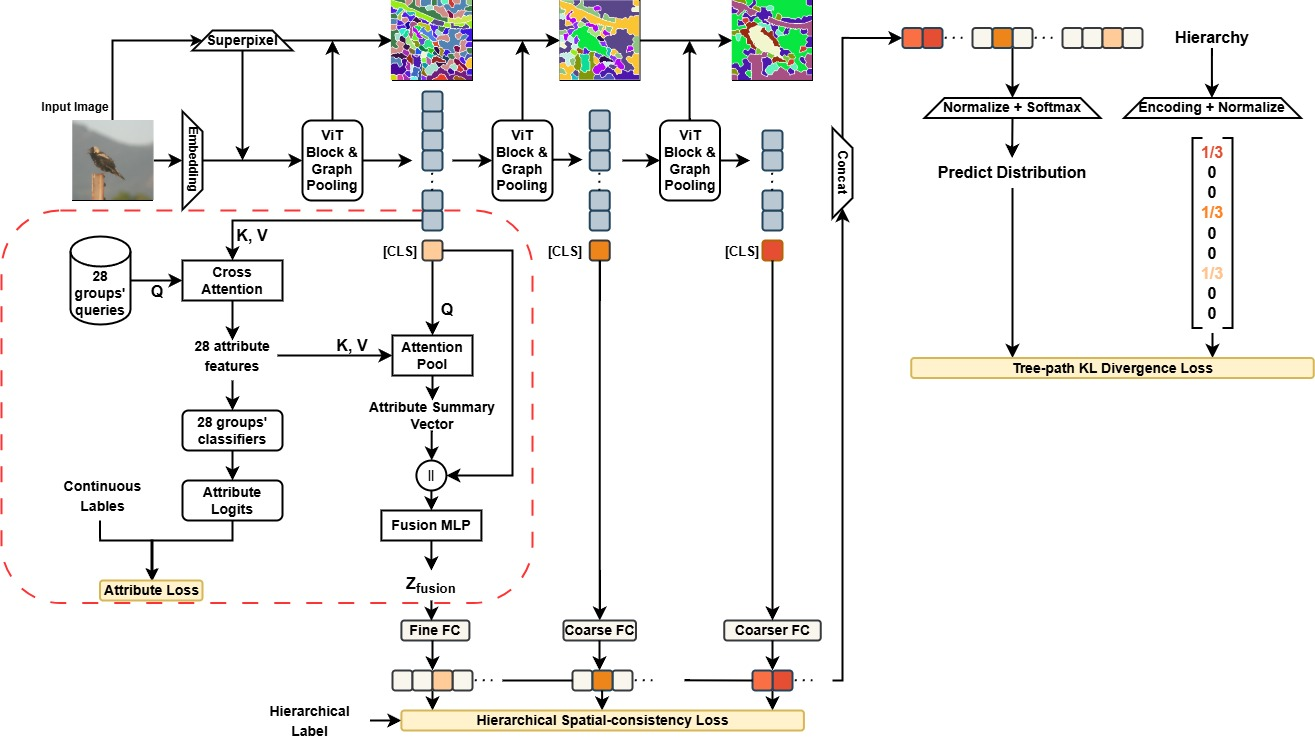
\includegraphics[width=\textwidth]{figures/proposed_overview.jpg}
    \caption{Overview of the proposed attribute-guided hierarchical bird classification framework. The H-CAST backbone extracts hierarchical visual representations from the input image. Attribute-group queries attend to species-level graph-node features and produce attribute-oriented representations. These representations are supervised by group-specific attribute prediction heads and fused with the species-level class token for final species prediction. Family and order predictions are produced from the original H-CAST hierarchy. Attribute labels are used only during training.}
    \label{fig:proposed_overview}
\end{figure}

The main addition of this thesis is an attribute-guided module attached to the species-level branch. This design is motivated by the nature of fine-grained bird recognition. Many difficult species-level errors occur between visually similar species, especially species within the same family. Such species may share global appearance but differ in subtle semantic traits such as bill shape, crown color, wing pattern, breast markings, or tail shape. These traits are directly described by CUB attributes \cite{wah2011cub}. Therefore, instead of relying only on taxonomy labels, the proposed model uses CUB attributes as auxiliary semantic supervision during training.

The attribute-guided module operates at the level of attribute groups rather than treating all 312 CUB attributes as a single flat output vector. The attributes are organized into semantic groups based on their names, such as bill shape, wing color, head pattern, breast color, and tail shape. For each active attribute group, the model maintains a learnable attribute-group query. These queries attend to the graph-node features from the species-level stage of H-CAST and produce attribute-oriented representations. Each representation is passed to a group-specific classifier, which predicts the retained attribute category within that group. These predictions are used as auxiliary outputs during training.

In addition to auxiliary attribute prediction, the proposed model uses the learned attribute-oriented features to support species classification. The attribute features are aggregated through an attention-pooling mechanism conditioned on the species-level visual representation. The resulting attribute summary is concatenated with the species class token and passed through a fusion module before the final species classifier. In this way, the species prediction can use both the image representation learned by H-CAST and the attribute-oriented representation learned from semantic supervision.

An important design choice is that attribute-guided fusion is applied primarily to the species-level branch. This is consistent with the role of attributes in fine-grained recognition: semantic traits are expected to be most useful for distinguishing visually similar species, while family and order labels correspond to coarser taxonomic levels. Therefore, the proposed model preserves the original H-CAST predictions for family and order. Although these higher-level classifiers are not directly fused with attribute features, they are still trained jointly with the species branch in the hierarchical classification framework.

To evaluate whether attribute-query cross-attention is necessary, this thesis also considers a direct-fusion baseline without cross-attention. In that baseline, group-wise attribute features are generated directly from the species class token and fused with the species representation. This baseline keeps the same image-only inference setting and the same auxiliary attribute supervision, but removes the cross-attention operation between attribute-group queries and species-level graph nodes. This comparison is used to determine whether the proposed cross-attention design provides additional benefit beyond simple feature fusion and model capacity.

Since CUB provides 312 attributes, using all attributes may introduce redundancy or weakly useful supervision. To address this issue, this thesis studies several attribute usage and selection strategies. The main proposed strategy, Hard-Sibling Discriminative Attribute Selection (HSDAS), selects attributes that help distinguish a species from its sibling species within the same family, with emphasis on hard siblings that have similar attribute profiles. The selected attributes define the active attribute groups used by the attribute prediction heads and the attribute-guided fusion module.

The model is trained with a combination of hierarchical classification loss, optional Tree-Path KL divergence, auxiliary attribute prediction loss, and optional attribute attention diversity regularization. The hierarchical classification loss follows the H-CAST setting and supervises predictions at species, family, and order levels. The attribute prediction loss supervises the group-specific attribute heads using selected group-wise attribute targets. For the cross-attention-based model, the diversity term is used as a regularization principle to reduce redundancy among macro-part-level attribute attention patterns. It is not intended to evaluate or guarantee pixel-level attribute localization.

During inference, the model remains image-based. No manually provided attribute labels are required. Given an input image, the H-CAST backbone extracts hierarchical visual features, the attribute-guided module internally produces attribute-oriented representations, and the fused species representation is used for species prediction. The model also outputs family and order predictions from the original H-CAST hierarchy. Thus, attributes are used to guide representation learning during training, while the final prediction pipeline remains compatible with standard image-only classification.

Overall, the proposed method combines three components: a visually consistent H-CAST backbone, attribute-guided species-level feature learning, and hard-sibling-aware attribute selection. The goal is to improve fine-grained species discrimination while preserving hierarchical prediction across species, family, and order.